\documentclass[10pt,a4paper]{article}
\usepackage[utf8]{inputenc}
\usepackage[english]{babel}
\usepackage[T1]{fontenc}
\usepackage{amsmath}
\usepackage{amsfonts}
\usepackage{amssymb}
\usepackage[math]{cellspace}
\usepackage{graphicx}
\usepackage[left=2cm,right=2cm,top=2cm,bottom=2cm]{geometry}
\DeclareMathOperator{\sinc}{sinc}

\title{Diffraction of light by any opening}
\author{PLASSE Jonathan, ROUSSEL Loïc, ROHR Julien, NAÏLI Kamel}

\begin{document}
\maketitle

\section{History of Diffraction}
The diffraction is a phenomenon discovered in 1665 by Francesco Maria Grimaldi. This physicist, whose interest lied in optics and astronomy, enjoyed drilling tiny openings in a black curtain exposed to the sun. He used these sources of improvised light and interposed on the path of the beam either slots of different shape or hair or even feathers of birds. Each time, he observed on a screen placed behind these objects, iridescent fringes located apart from the normal geometrical route. He then made the assumption that the change in trajectory of the light -caused by the presence of an hurdle or an opening- was the manifestation of a new phenomenon, namely the diffraction. His discovery was published in 1665 -after his death- in "Physicomathesis de lumine, coloribus, et iride".

Christian Huygens ( 1629-1695 ) was also interested in this new phenomenon. In 1690 is published "Trait\'e de la lumi\`ere" in which he lays down the foundations for the undulatory theory of the light. By likening light with waves on the surface of water and the sound waves in the air, he assumed that light propagated in a spherical pattern -thus leading to the concept of wave of light-, and that every point reached by the wave behaved as a new source called "secondary source". However, his analogy went too far, since he believed that light vibration was longitudinal and needed a material medium to propagate. Unable to define exactly the nature of this medium, he called it "the ether". 

The theory of wavelets allowed him to find the law of Snell-Descartes for refraction. This theory was complemented by Isaac Newton ( 1642-1727 ), who also observed diffraction and the localized fringes infered by thin blades but developed a corpuscular theory. 

After the highlighting of interference fringes by his famous double slots, Thomas Young (1773-1829) relaunched the undulatory theory of light. Augustin Fresnel (1788-1827) imagined two new devices to obtain interferences -mirrors and biprism- and generalized the approach of Huygens. The resulting principle of Huygens-Fresnel allows finding accurately the diffraction pattern whatever the shape of the slot is, given one can solve the calculus involved. 

Fraunhofer is mostly known for inventing the spectroscope in 1814 and thanks to it discovering absorption rays in the solar spectrum. Besides this, he was the first to study the diffraction of light by optical gratings, which he used to measure accurately the optical properties of glasses (refractive index). He also gave his name to the far field diffraction pattern analysis. 

The equations of James-Clerk Maxwell (1831-1879) on electromagnetism support the wave theory of light, but it was not until Albert Einstein introduced quantum physics in 1905 and reestablished a corpuscular aspect that the two theories were brought together.

\section{The diffraction regimes}
	\subsection{Fresnel diffraction}
Fresnel diffraction also known as near field diffraction is a description of the physical diffraction phenomenon when observed close to the diffractive object. It takes into account the curvature of the wavefront, and therefore the variation of the phase term resulting from the propagation in the spherical shape of the light in accordance with the principle of Huygens-Fresnel. For each point of the space -which are considered independent-, the reception of a wave of given magnitude, frequency and phase triggers the repetition of a spherical wave of the same magnitude, frequency and phase. Instead of considering that the wave progresses continuously, its progression is decomposed by imagining that it is progressing step by step. The diffraction pattern arising from any slot will be an integration calculation. 

The equation of propagation of a spherical wave is:

\[E(r,t)= \frac{E_0}{r} \exp\left(j(kr-\omega t)\right)\]

The elementary variation of E(r,t) by the principle of Huygens-Fresnel:

\[\mathrm{d}E=\frac{\exp\left(jkr\right)}{r} E(x',y') \mathrm{d}x' \mathrm{d}y'\]

By the use of the Helmoltz equation in a homogeneous medium: 

\[\Delta E+k^2 E=0\]

And by integration on the surface of the opening of the slot, we obtain:

\[
E(x,y)=\frac{1}{j\lambda}
\times \iint \frac{\exp\left(jkr\right)}{r}
E(x',y')\mathrm{d}x'\mathrm{d}y'
\]

	\subsection{The diffraction of Fraunhofer}
The Fraunhofer diffraction is an approximation of far field diffraction, i.e. observation at a great distance from the diffractive object. The radius of curvature of the diffracted waves is therefore very large, so that they can be considered as plane waves. This approximation can also be used when the diffraction pattern is observed in the image focal plane of a converging lens. The advantage is that it allows one to go through a Fourier transform calculation, which is more often than not easier than going through the integration calculus.

\begin{center}
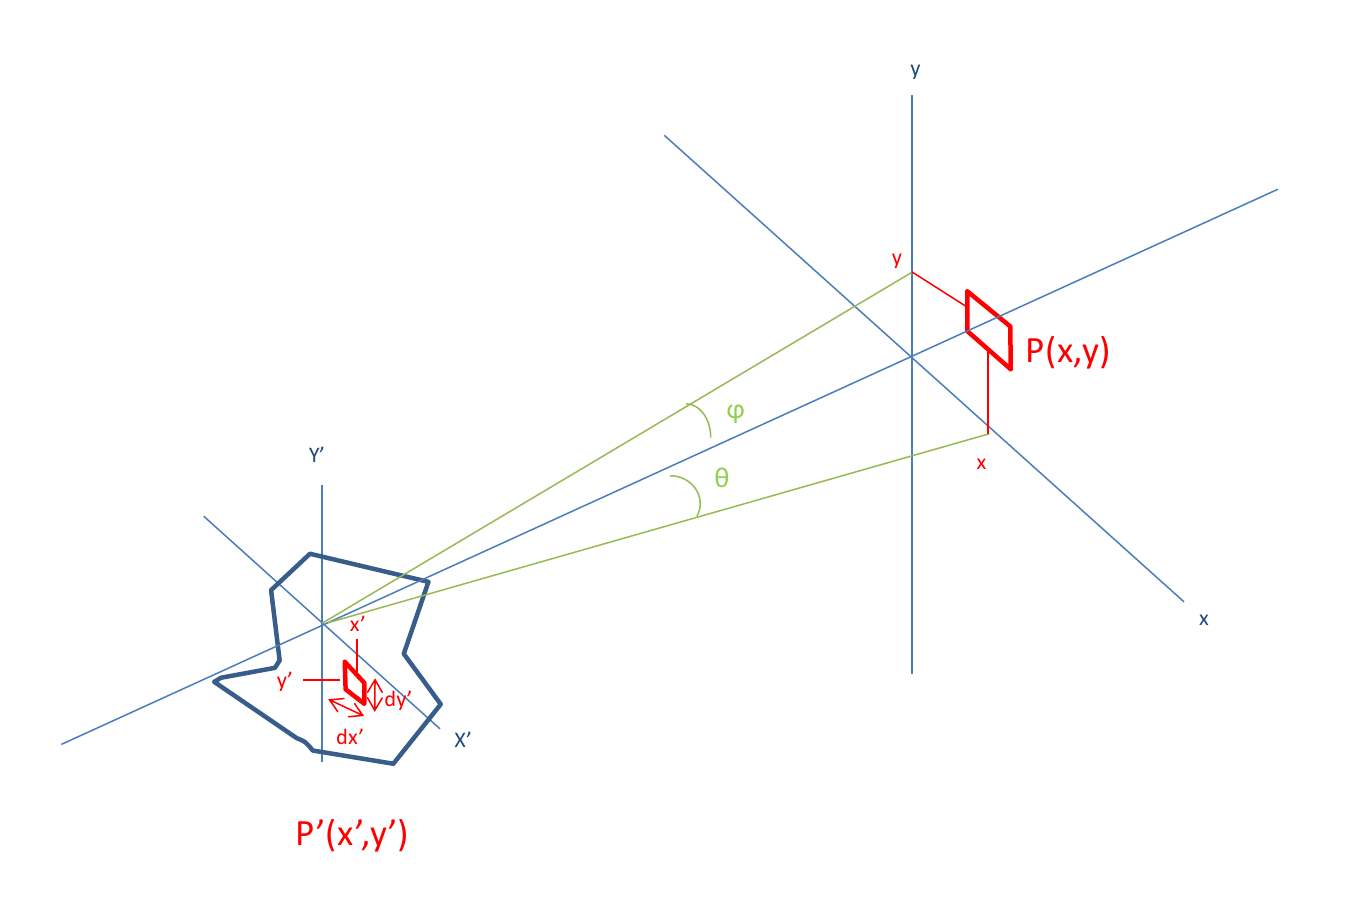
\includegraphics[scale=0.32]{./figures/schema-1-crop.png}
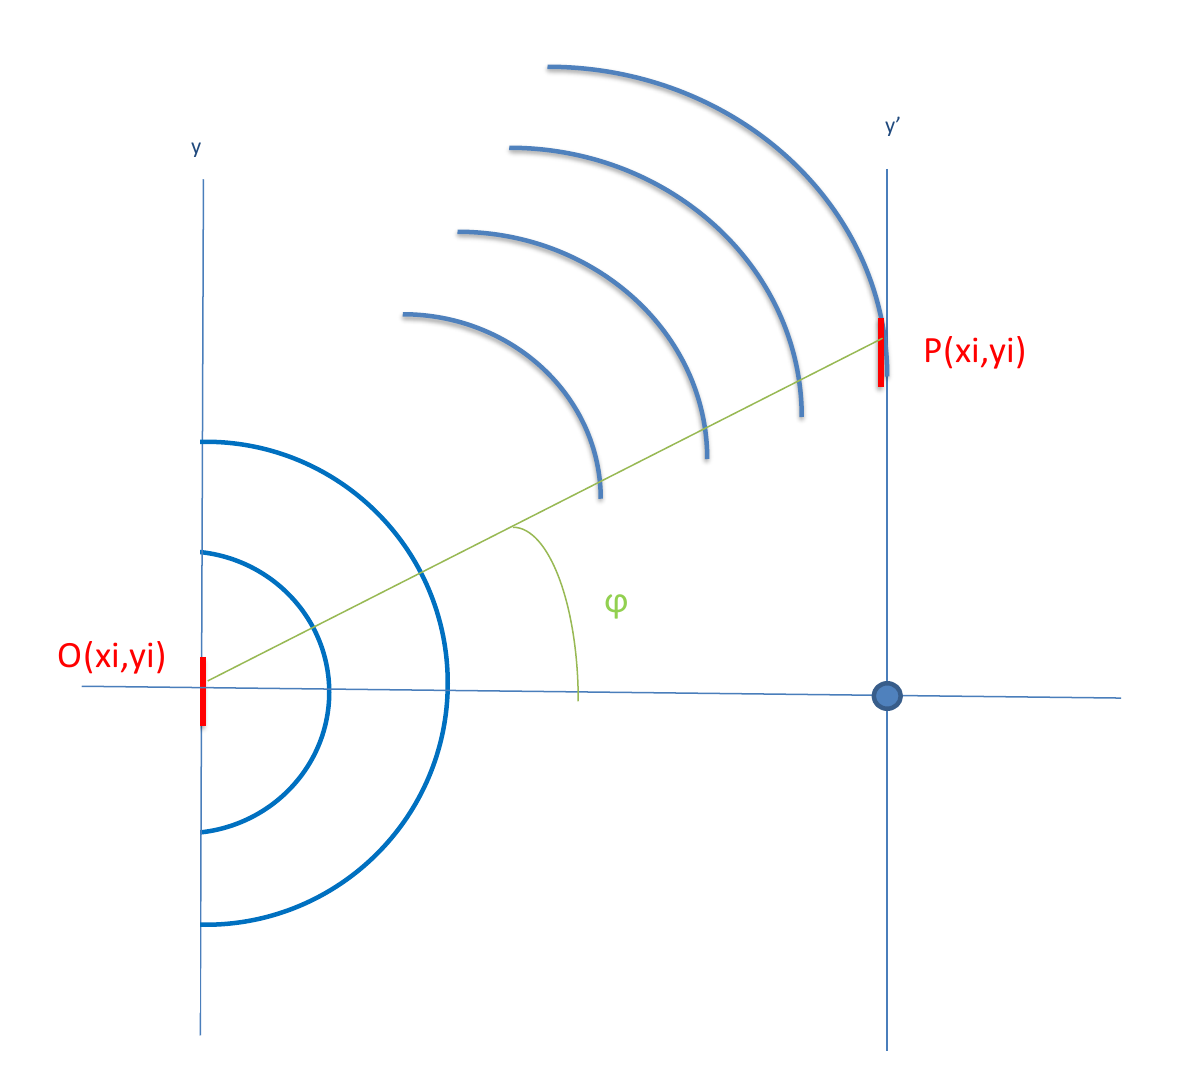
\includegraphics[scale=0.32]{./figures/schema-2-crop.png}
\end{center}

\[r=\sqrt{z^2+(x-x')^2+(y-y')^2}\]
\[r=z\sqrt{1+\left(\frac{x-x'}{z}\right)^2+\left(\frac{y-y'}{z}\right)^2}\]

In Fraunhofer’s regime:

\[z^2\gg(x-x')^2+(y-y')^2\]

We can carry out a development limited to order 1: 

\[r=z\left(1+\frac{1}{2}\left(\frac{x-x'}{z}\right)^2+\frac{1}{2}\left(\frac{y-y'}{z}\right)^2\right)\]

After development:

\[r \approx z+\frac{x^2+y^2}{2z}+\frac{x'^2+y'^2}{2z}-\frac{xx'+yy'}{z}\]

This approximation is still valid in the Fresnel region. 

If we are very far from the source, the last term becomes negligible and we find ourselves in the Fraunhofer region.

\begin{center}
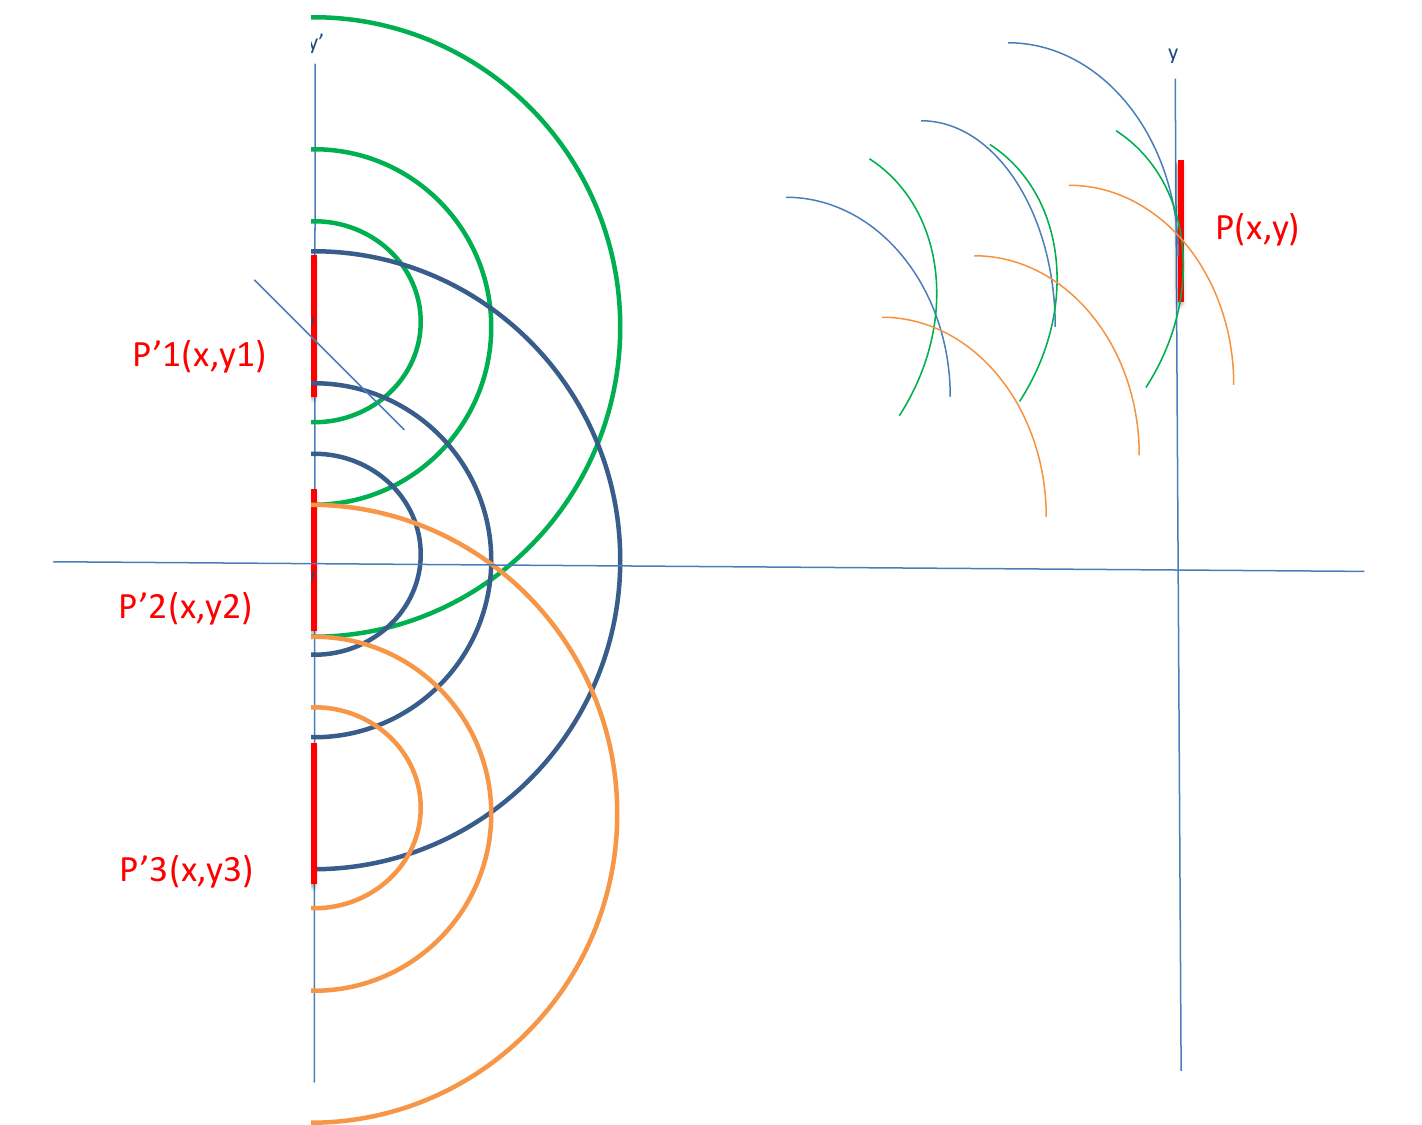
\includegraphics[scale=0.32]{./figures/schema-3-crop.png}
\end{center}

\[r \approx z+\frac{x^2+y^2}{2z}-\frac{xx'+yy'}{z}\]

\[
E(x,y)=\frac{1}{j\lambda} 
\times \iint \frac{\exp\left(jkr\right)}{r}
E(x',y')\mathrm{d}x'\mathrm{d}y'
\]

With $r\approx z$ at the denominator for the damping term of the wave and $r \approx z+\frac{x^2+y^2}{2z}-\frac{xx'+yy'}{z}$ for the term of phase:

\[
E(x,y)=\frac{1}{j\lambda z} \exp\left(jk\left(z+\frac{x^2+y^2}{2z}\right)\right)
\times \iint \exp\left(-jk\frac{xx'+yy'}{z}\right)
E(x',y')\mathrm{d}x'\mathrm{d}y'
\]

Let $f_x=\frac{x}{\lambda z}$ and $f_x=\frac{y}{\lambda z}$

\[
E(x,y)=\frac{1}{j\lambda z} \exp\left(jk\left(z+\frac{x^2+y^2}{2z}\right)\right)
\times \underbrace{
	\iint \exp\left(-2\pi j(f_xx'+f_yy')\right)E(x',y')\mathrm{d}x'\mathrm{d}y'
}_\text{Fourier's transformation}
\]

Polar coordinates in the Fraunhofer regime:

\[x=\rho \cos(\omega) \]
\[y=\rho \sin(\omega) \]
\[x'=\rho \cos(\omega') \]
\[y'=\rho \sin(\omega') \]

Elementary area: $\mathrm{d}x\mathrm{d}y=\rho \mathrm{d}\rho \mathrm{d}\omega$

So, we use the expression Cartesian:

\[
\begin{array}{rcl}
E(\rho,\omega) & = & \frac{1}{j\lambda z} \exp\left(jk\left(z+\frac{\rho^2 \cos(\omega)^2+\rho^2 \sin(\omega)^2}{2z}\right)\right)\\
& & \times \iint \exp\left(-jk\frac{\rho \cos(\omega)\rho' \cos(\omega')+\rho \sin(\omega)\rho' \sin(\omega)'}{z}\right)
E(\rho',\omega')\rho' \mathrm{d}\rho'\mathrm{d}\omega'
\end{array}
\]

\[
E(\rho,\omega)=\frac{1}{j\lambda z} \exp\left(jk\left(z+\frac{\rho^2}{2z}\right)\right)
\times \iint \exp\left(-jk\frac{\rho\rho'\cos(\omega-\omega')}{z}\right)
E(\rho',\omega')\rho' \mathrm{d}\rho'\mathrm{d}\omega'
\]

\section{Fraunhofer case study}
	\subsection{Rectangular opening}
\[
\left \{
\begin{array}{r c l}
x' & \in & \left[-\dfrac{a}{2};\dfrac{a}{2}\right]\\
y' & \in & \left[-\dfrac{b}{2};\dfrac{b}{2}\right]
\end{array}
\right .
\]

For a rectangular opening E(x’,y’)= 1 only if

\begin{center}
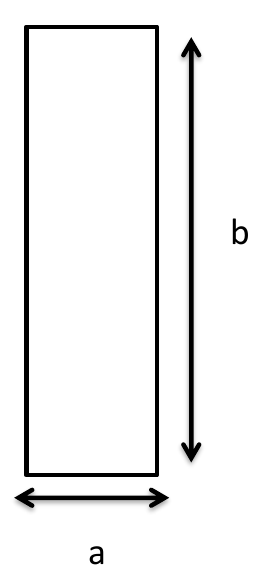
\includegraphics[scale=0.3]{./figures/schema-4-1.png}
\end{center}

\[
E(x,y)=\frac{1}{j\lambda z} \exp\left(jk\left(z+\frac{x^2+y^2}{2z}\right)\right)
\times \int_{-\frac{a}{2}}^\frac{a}{2} \int_{-\frac{b}{2}}^\frac{b}{2}
 \exp\left(-2\pi j(f_xx'+f_yy')\right)\mathrm{d}x'\mathrm{d}y'
\]

Separation of variables:

\[
E(x,y)=\frac{1}{j\lambda z} \exp\left(jk\left(z+\frac{x^2+y^2}{2z}\right)\right)
\times \int_{-\frac{a}{2}}^\frac{a}{2} \exp\left(-2\pi jf_xx'\right)\mathrm{d}x'
\times \int_{-\frac{b}{2}}^\frac{b}{2} \exp\left(-2\pi jf_yy'\right)\mathrm{d}y'
\]

After Fourier’s transformation:

\[
E(x,y)=\frac{1}{j\lambda z} \exp\left(jk\left(z+\frac{x^2+y^2}{2z}\right)\right)
\times a\sinc\left(2\pi f_x \frac{a}{2}\right)
\times b\sinc\left(2\pi f_y \frac{b}{2}\right)
\]

	\subsection{Plane wave}
For a plane wave:

\[E(x',y')=A\exp\left(j(\omega t-kz)\right)\]

\[
E(x,y)=\frac{1}{j\lambda z} \exp\left(jk\left(z+\frac{x^2+y^2}{2z}\right)\right)
\times \iint \exp\left(-2\pi j(f_xx'+f_yy')\right)
A\exp\left(j(\omega t-kz)\right)\mathrm{d}x'\mathrm{d}y'
\]

\[
E(x,y)=\frac{1}{j\lambda z} \exp\left(jk\left(z+\frac{x^2+y^2}{2z}\right)\right) A\exp\left(j(\omega t-kz)\right)
\times \underbrace{
	\iint \exp\left(-2\pi j(f_xx'+f_yy')\right)
	\mathrm{d}x'\mathrm{d}y'
}_\text{divergent term}
\]

The term divergent says that all the image plane is received by light, there is not really any phenomenon of diffraction (no principle of causality $\Rightarrow$ diffraction if there is a cause to it: here it does not there is not any). Limit case that confirming the model.

	\subsection{Narrow slot}
For a slot, we have the case of a rectangular opening except that $a\rightarrow 0$.

Thus
	
\[
E(x,y)=\frac{1}{j\lambda z} \exp\left(jk\left(z+\frac{x^2+y^2}{2z}\right)\right)
\times \lim_{a\rightarrow 0} \iint\limits_S \exp\left(-2\pi j(f_xx'+f_yy')\right)\mathrm{d}x'\mathrm{d}y'
\]

\[
E(x,y)=\frac{1}{j\lambda z} \exp\left(jk\left(z+\frac{x^2+y^2}{2z}\right)\right)
\times \int_{-\frac{b}{2}}^\frac{b}{2} \exp\left(-2\pi jf_yy'\right)\mathrm{d}y'
\times \lim_{a\rightarrow 0} \int_{-\frac{a}{2}}^\frac{a}{2} \exp\left(-2\pi jf_xx'\right)\mathrm{d}x'
\]

\[
E(x,y)=\frac{1}{j\lambda z} \exp\left(jk\left(z+\frac{x^2+y^2}{2z}\right)\right)
\times b\sinc\left(2\pi f_y \frac{b}{2}\right)
\times \lim_{a\rightarrow 0}a\sinc\left(2\pi f_x \frac{a}{2}\right)
\]

\[
E(x,y)=\frac{1}{j\lambda z} \exp\left(jk\left(z+\frac{x^2+y^2}{2z}\right)\right)
\times b\sinc\left(2\pi f_y \frac{b}{2}\right)
\times \epsilon
\]

	\subsection{Circular opening}
\begin{center}
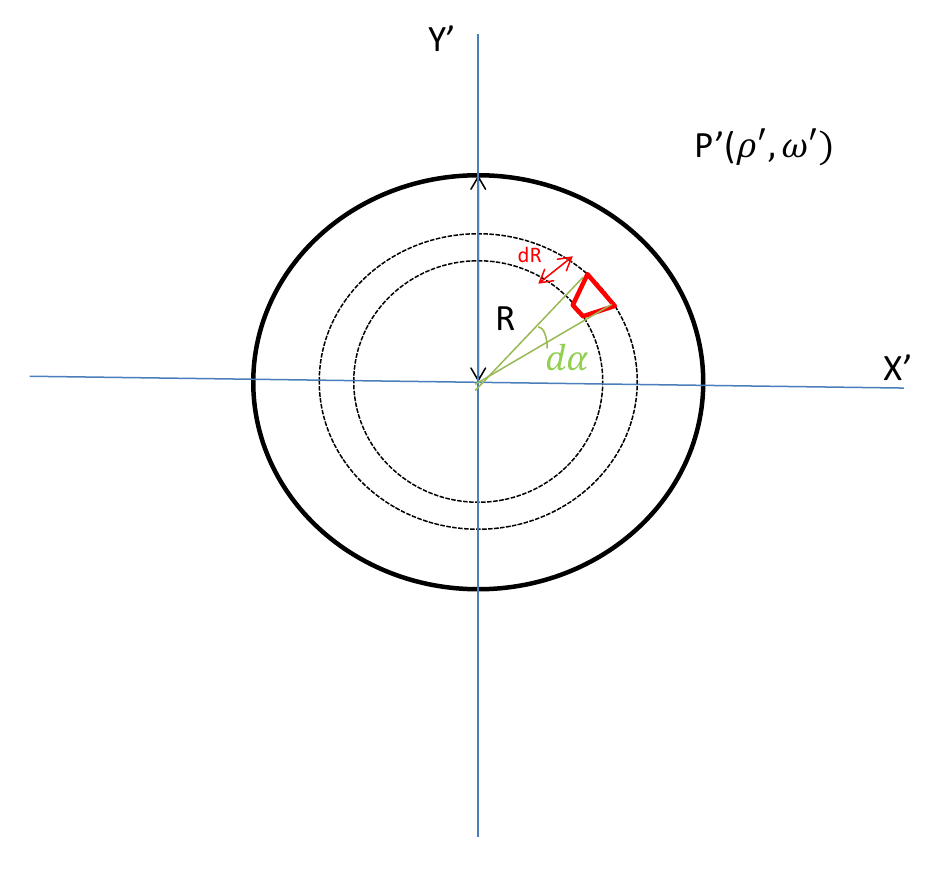
\includegraphics[scale=0.3]{./figures/schema-4-2.png}
\end{center}

\[
E(\rho,\omega)=\frac{1}{j\lambda z} \exp\left(jk\left(z+\frac{\rho^2}{2z}\right)\right)
\times \iint \exp\left(-jk\frac{\rho\rho'\cos(\omega-\omega')}{z}\right)
E(\rho',\omega')\rho' \mathrm{d}\rho'\mathrm{d}\omega'
\]

\[
E(\rho,\omega)=\frac{1}{j\lambda z} \exp\left(jk\left(z+\frac{\rho^2}{2z}\right)\right)
\times \int_0^R \int_0^{2\pi} \exp\left(-jk\frac{\rho\rho'\cos(\omega-\omega')}{z}\right)
\rho' \mathrm{d}\rho'\mathrm{d}\omega'
\]

Let $u=-\frac{k\rho\rho'}{z}$, $\varphi=\omega-\omega'$ and $\nu=-\frac{k\rho R}{z}$.

\[
E(\rho,\omega)=\frac{1}{j\lambda z} \exp\left(jk\left(z+\frac{\rho^2}{2z}\right)\right)
\left(\frac{z}{k\rho}\right)^2
\times \int_0^\nu \int_0^{2\pi} \exp\left(ju\cos(\varphi)\right)
u \mathrm{d}u\mathrm{d}\varphi
\]

Then we use the following Bessel integral:

\[J_0(u)=\frac{1}{2\pi}\int_0^{2\pi} \exp\left(ju\cos(\varphi)\right)\mathrm{d}\varphi\]

We obtain:

\[
E(\rho,\omega)=\frac{1}{j\lambda z} \exp\left(jk\left(z+\frac{\rho^2}{2z}\right)\right)
\left(\frac{z}{k\rho}\right)^2
\times 2\pi \int_0^\nu u J_0(u) \mathrm{d}u
\]


Since $\nu J_1(\nu)=\int_0^\nu u J_0(u) \mathrm{d}u$  :

\[
E(\rho,\omega)=\frac{k}{jz} \exp\left(jk\left(z+\frac{\rho^2}{2z}\right)\right)
\left(\frac{z}{k\rho}\right)^2
\times \nu J_1(\nu)
\]

$J_1$ is an odd function so:

\[
E(\rho,\omega)=\frac{k}{jz} \exp\left(jk\left(z+\frac{\rho^2}{2z}\right)\right)
\left(\frac{z}{k\rho}\right)^2
\times \frac{k\rho R}{z} \times J_1\left(\frac{k\rho R}{z}\right)
\]

\[
E(\rho,\omega)=\frac{R}{j\rho} \exp\left(jk\left(z+\frac{\rho^2}{2z}\right)\right)
J_1\left(\frac{k\rho R}{z}\right)
\]

\section{FFT Explaination}
	\subsection{Theory}
Fourier analysis is fundamentally a method for expressing a function as a sum of periodic components, and for recovering the function from those components. When both the function and its Fourier transform are replaced with discretized counterparts, it is called the discrete Fourier transform (DFT). The DFT is in general defined for complex inputs and outputs. 

There are many ways to define the DFT. In the implementation of Python, the DFT is defined as

\[A_k=\sum_{m=0}^{n-1}a_m\left\lbrace-2\pi i\frac{mk}{n}\right\rbrace\
\quad
k\in[0;n[\]

As far as normalisation is concerned ,the default normalization has the direct transforms unscaled. 

The fast Fourier transform (FFT) is an algorithm for calculating discrete Fourier transform (DFT).Its complexity varies in $O(n\log n)$ with the number n of points used while a current DFT varies in $O(n^2)$. The calculation time of the fast algorithm can be 100 times shorter than the calculation using the DFT definition formula 

In 1965, James Cooley and John Tukey, two mathematicians in signal processing, published an fundamental article dealt with Fast Fourier transform and infered the massive adoption of this method. This method became mainstream in the field of digital signal processing and telecommunication.  

This algorithm is commonly used to transform discrete time domain data in the frequency domain, particularly in spectrum analyzers. Its efficiency makes it possible to carry out filtering by modifying the spectrum.  

Because the discrete Fourier transform separates its input into components that contribute at discrete frequencies, using a list where each discretization are gathered seems to be convenient. 

That's hinges on a function pulled out from a package called numpy in Python : $fft(a)$ with a an array (can be complex). 

If a array $A$ defined as $fft(a)$, then $A[0]$ contains the zero-frequency term (the sum of the signal), which is always purely real for real inputs. Then $A\left[1:\frac{n}{2}\right]$ contains the positive-frequency terms, and $A\left[\frac{n}{2}+1:\right]$ contains the negative-frequency terms, in order of decreasingly negative frequency. For an even number of input points, $A\left[\frac{n}{2}\right]$ represents both positive and negative Nyquist frequency, and is also purely real for real input. For an odd number of input points, $A\left[\frac{n-1}{2}\right]$ contains the largest positive frequency, while $A\left[\frac{n+1}{2}\right]$ contains the largest negative frequency. 

To return an array whose frequencies are corresponding with elements in the output, the function $fftfreq()$ should be harnessed. Otherwise, $fftshift()$ is a routine to shift transforms and their frequencies to put the zero-frequency components in the middle. 

Inasmuch as in this project, array in two dimensions needed to depict the diffraction patterns, a FFT allowing in argument this kind of array is regarded as a blessing. Numpy afford a function called $fft2()$ which fills out the job.  

In two dimensions, the DFT is defined as 

\[A_{kl}=\sum_{m=0}^{M-1}\sum_{n=0}^{N-1}a_{mn}\left\lbrace-2\pi i\left(\frac{mk}{M}+\frac{nl}{N}\right)\right\rbrace\
\quad
k\in[0;M[l\in[0;N[\]

	\subsection{About the diffraction figure scaling}
\[
\begin{array}{ccc}
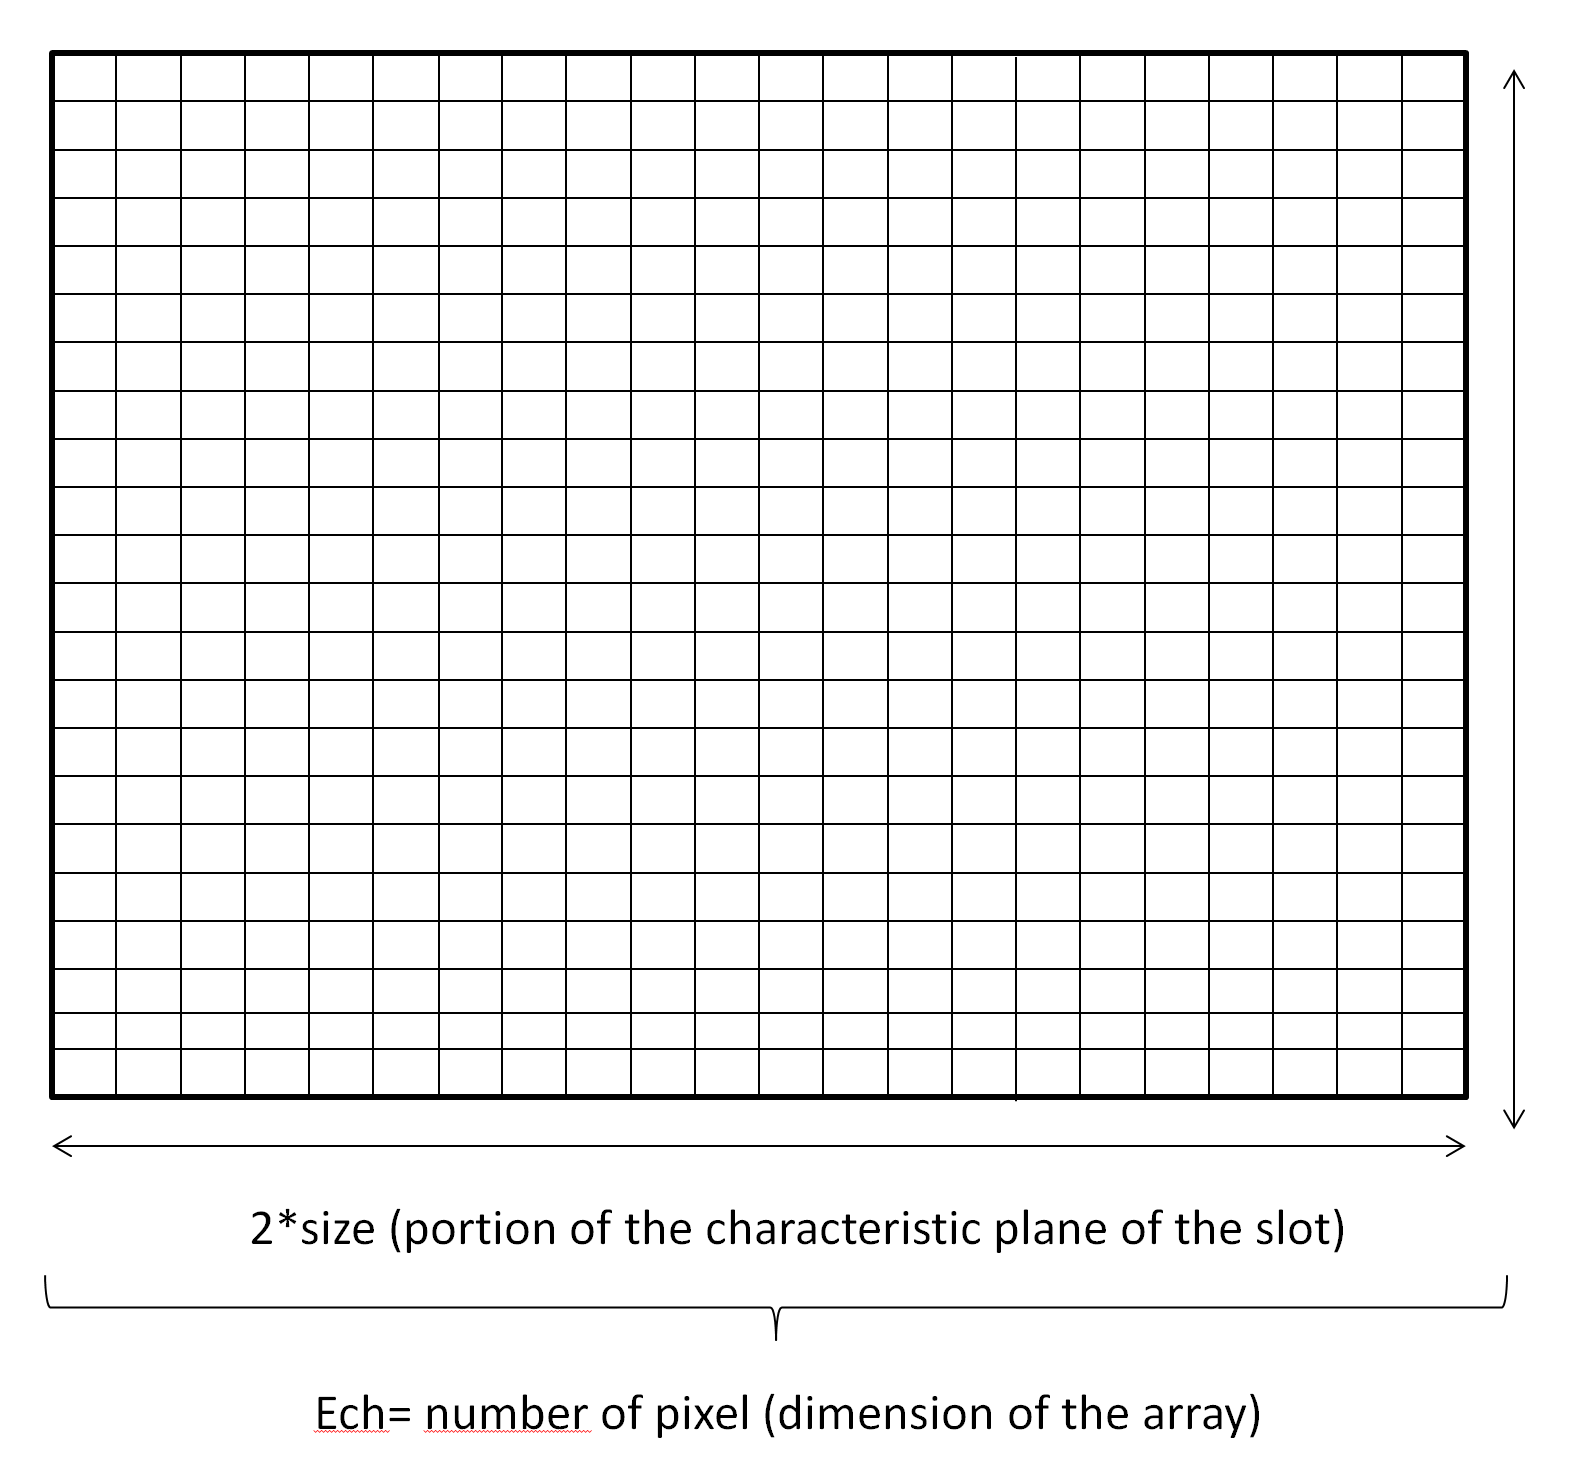
\includegraphics[scale=0.1]{./figures/schema-5-1-crop.png} &
\substack{\rightarrow\\
z\text{(distance between the planes)}\\
\rightsquigarrow\\
\lambda\text{(wavelength)}}
& 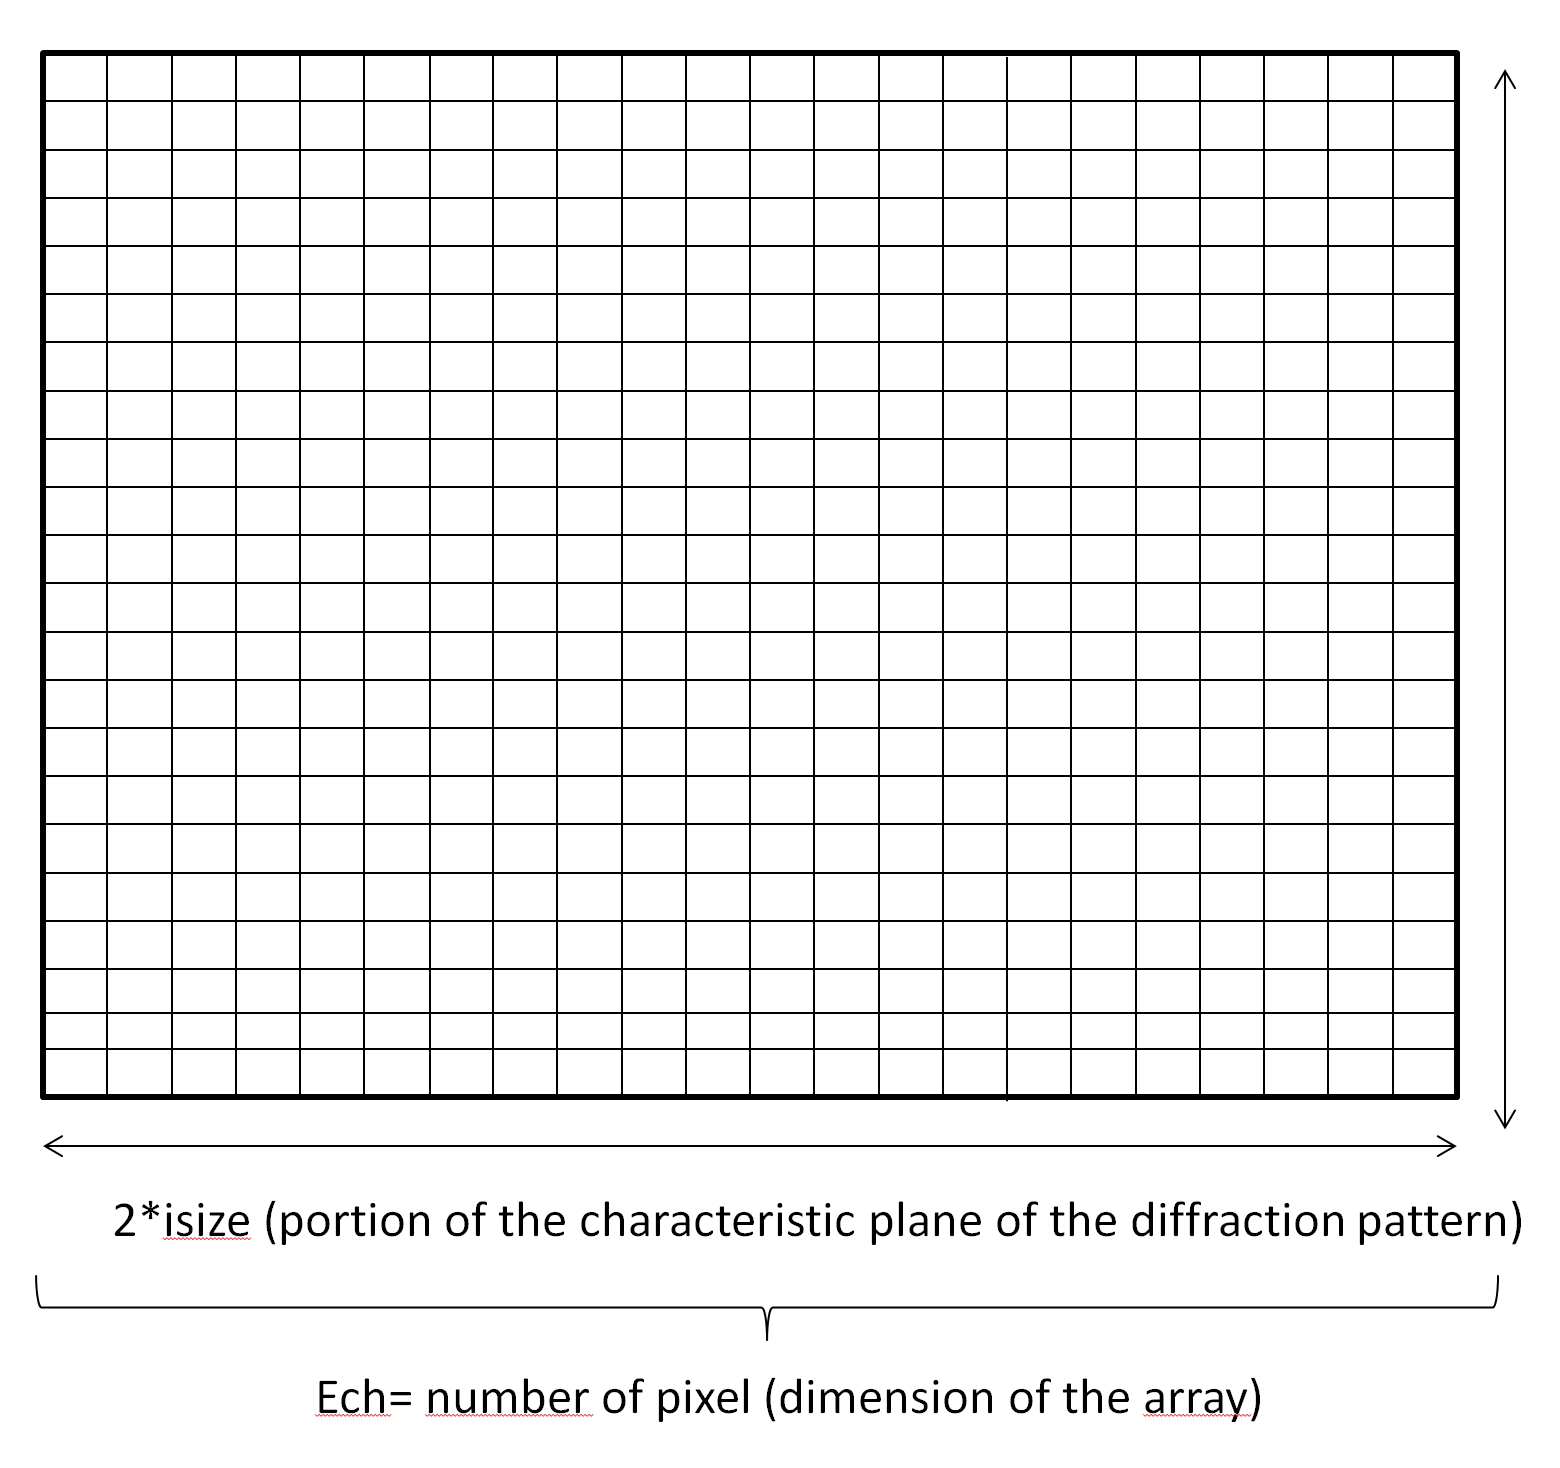
\includegraphics[scale=0.1]{./figures/schema-5-2-crop.png}
\end{array}
\]

The diffraction by an elementary aperture, i.e. a pixel, is described by
$\sin(\theta)= \frac{\lambda}{a}$  with a the characteristic size of the aperture. 

Considering a plane orthogonal to the propagation axis $z$ and thus containing the $x$ and $y$ axis, we obtain by projecting on the axis $x$ for instance :

\[\sin(\theta)=\frac{\mathrm{d}x}{\mathrm{d}z}\]

Thus :

\[\frac{\mathrm{d}x}{\mathrm{d}z}= \frac{\lambda}{a}\]

And thus :

\[\frac{\Delta x}{\Delta z}= \frac{\lambda}{a}\]

With the notations used before, $a=2size$, $\Delta x=2i_{size}$ (for one pixel) and $\Delta z = z$

Thus :
\[\frac{i_{size}\text{ (for one pixel)}}{z}=\frac{\lambda}{size}\]

Thus :
\[i_{size}\text{ (for one pixel)}=\frac{\lambda z}{size}\]

Since there are $(ech-1)$ pixels on one line of the image, we obtain :
\[i_{size}\text{ (whole image)}=\frac{\lambda z}{size}(ech-1)\]
\end{document}}
